\section{Restaurant}
The robot is tested in a real environment such as a real restaurant or a shopping mall.

\subsection{Focus}
This test focuses on online mapping, safe navigation in previously unknown environments, gesture detection, human-robot interaction, and manipulation in a real environment.

The robot will need to create its own map from the environment and then move into it to handle human requests, such as delivering drinks or snacks, while people are walking around.

\subsection{Setup}
\begin{enumerate}
	\item \textbf{Location:} A real restaurant fully equipped with a \quotes{Professional Waiter} and at least three tables with \quotes{Professional Clients}. 
\end{enumerate}

\subsection{Task}
\begin{enumerate}
	\item \textbf{Instruction:} In case the robot can work with a \quotes{Professional Waiter}, the team should very briefly instruct the waiter how to command the robot, e.g. what to say when a table location must be memorized etc.
	
	\item \textbf{Start:} The robot starts at a designated starting position, and waits for an operator: the \quotes{Professional Waiter}. When the referees start the time, the team is allowed to (briefly) instruct the operator. After the instruction, the operator steps in front of the robot and tells it to follow (no start signal).

	\item \textbf{Memorizing the operator:} The robot has to memorize the operator. During this phase, the robot may instruct the operator to follow a certain setup procedure.

	\item \textbf{Guide phase:} Starting from the \textit{Kitchen}, the robot is guided through the environment by a \quotes{Professional Waiter} which shows to the robot the location of each of the tables, its number, and on which side the table is (there is a total of 3 tables). After visiting all the tables, the robot must be guided again to the \textit{Kitchen}, to the same place where the guide phase started.

	\begin{itemize}
		\item \textbf{Own \textit{Professional Waiter} [Optional]:} Team Leader may choose to use their own custom \textit{Professional Waiter} for this test instead of the one provided by the committee.
		\item \textbf{Finding the tables [Optional]:} Team Leader may choose not to tell the robot on which side (left or right) is the table, and let the robot find the tables by itself. When using this option, the robot must state where the table is (e.g.~by telling: \textit{the table is to my right}).
	\end{itemize}
	\textbf{Remark:} When using a custom \textit{Professional Waiter}, no points are earned for state the side of the table.

	\item \textbf{Ordering phase:}
	\begin{enumerate}
		\item \textbf{Which table to attend:} Once back in the kitchen, the robot shall ask to the \textit{Professional Waiter} to which table go first to take an order from. 
		  The robot has to go to the indicated table and ask for an order there.
		  This interaction of telling the robot which table to attend should be natural.
		  
		\item \textbf{First order (Table A)}: The robot must aks the person what he or she wants to order. See Orders below for details about ordering.

		\item \textbf{Detecting a call (Table B or C):} At any time while attending Table A's guests (going to fetch an order, asking the client, or returning to the kitchen with the order), a guest at Table B or C will ask for the robot's attention by waving \emph{and} calling it out using voice. 
		  The robot must state out loud that it has detected the call and that it will attend as soon as possible.
		  If the robot does not detect such a call, it may be given a command to go to the next table when it is back at the kitchen after finishing table A's order.

		\item \textbf{Second order (Table B or C):} After taking the Table A client's order, and if the request was detected, the robot must go to the table of the waving/calling person and ask for an order.
		  

		\item \textbf{Avoiding random citizen:} At any time while going to any of the tables or to the \textit{Kitchen}, a person may step on the robot's path. It is expected the robot to avoid that person or stop and wait for it to move away.
	\end{enumerate}

	\textbf{Orders:} The menu offers Beverages and Combos. An order may be a Beverage or Combo. One guest will order a Combo while the other will order a Beverage.
	  A Combo is a combination of two of the food items from the set of objects \ref{rule:scenario_objects}, e.g. ``noodles with peanuts'' or ``noodles and peanuts''. 
	  Guests also prefere to state their order in a natural way, as their would in a restaurant operated by humans. 

	\textbf{Note:} Table A, B and C may be any of Table 1, 2, 3, \dots, N in any order.

	\item \textbf{Delivering phase:}
	\begin{enumerate}
		\item \textbf{Repeating the order:} Once again in the kitchen, the robot recites the orders for each table, including the table number (e.g.~\textit{Hamburger with fries for table 1 and Orange juice for table 2}), to the \textit{Professional Barman}. This includes determining the table number of the waving/calling person. The \textit{Professional Barman} will serve the order and place it into a tray on the Kitchen-bar.
		  If the barman cannot understand the order that the robot repeats, he cannot hand out the order and no points can be awarded for reciting the order.

		\item \textbf{Delivering Beverage:} The robot must grab a can of the appropriate drink from a set of cans on the Kitchen-bar and deliver it to the correct table.

		\item \textbf{Delivering Combo:}  The robot must carry a tray with the ordering to the table the food was ordered from. Teams must indicate beforehand whether the robot is able to grasp the plate itself, whether it needs a tray or whether the plate needs to be handed to the robot.
	\end{enumerate}

	\item \textbf{Next customer, please:} The task is finished when the robot has delivered both orders and is back at the kitchen.
\end{enumerate}

\begin{figure}[tbp]
	\centering
	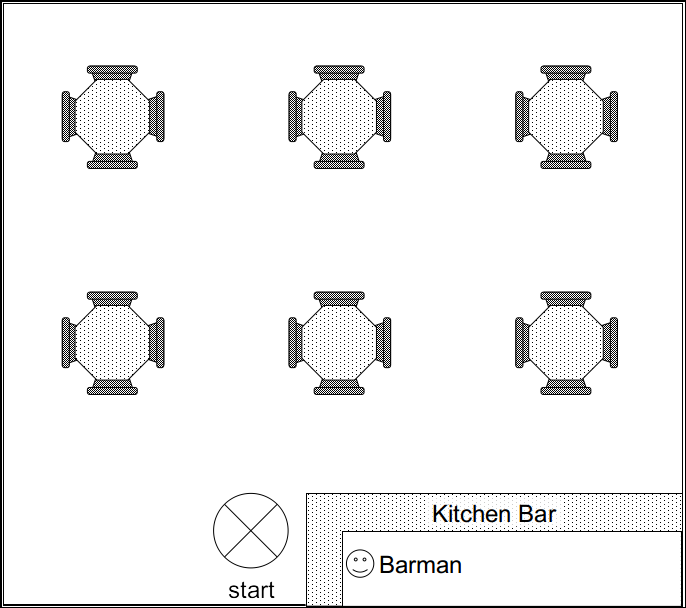
\includegraphics[width=0.5\columnwidth]{images/restaurant.png}
	\caption{Restaurant test: example setup.}
	\label{fig:restaurant}
\end{figure}

\subsection{Additional rules and remarks}

\begin{itemize}
	\item \textbf{Safety!} This test takes place in a public area. That is, there may be people standing, sitting or walking around the area throughout the test. The robot is expected to not even slightly touch anything and is immediately stopped in case of danger.

	\item \textbf{Referees and guidance:} For safety reasons, the referees in this test are TC members. One of the referees follows the robot and is always in reach of the emergency button.

	\item \textbf{Start:} There is no fixed start signal in this test.

	\item \textbf{Order:} The way the user provides information to the robot is up to the robot's team. A natural interaction is preferred.

	\item \textbf{Location:} This test can be arranged in any real restaurant or shopping mall. If this is not possible, the test can be conducted in an arbitrary room containing the appropriate locations. The only requirement is that this room is not part of the arena and that the teams do not know the room beforehand. The exact location, including the object and delivery locations, will be defined by the technical committee on site (and in corporation with the local organization). In addition, to avoid unnecessary time investment for navigation, the distances between tables and the ``Kitchen Bar'' will be minimal.

	\item \textbf{Natural walking:} The operator has to walk \quotes{naturally}, i.e., move forward facing forward. If not mentioned otherwise, the operator is not allowed to walk back, stand still, signal the robot or follow some recalibration procedure.

	\item \textbf{Disturbances from outside:} If a person from the audience (severely) interferes with the robot in a way that makes it impossible to solve the task, the team may repeat the test immediately.

	\item \textbf{Learning tables:} Of course, it can only be sure that a robot correctly learned a table when it is able to go there after being commanded so. 
	
	\item \textbf{Instruction:} The robot interacts with the operators, not the team. That is, the team is only allowed to (very!) briefly instruct the \textit{Professional Waiter} and \textit{Professional Barman} 
	\begin{itemize}
		\item how to the tell the robot to follow,
		\item how to visually/acoustically indicate table names and position (e.g., pointing or telling \quotes{Table 1 is on your left}), 
		\item how to the tell the robot the \textit{Guide Phase} has ended, and
		\item how to the tell the robot the order has been served
	\end{itemize}
	It is not allowed to the team to instruct the clients on how to get robot's attention. It shall be done in a natural way like when interacting with a human waiter.

	\item \textbf{Kitchen-bar:} The \textit{Kitchen-bar} will be a table located at the restaurant's kitchen, next to the place where the \textit{Guide Phase} started and ended. 
	The robot may ask on which side of the robot the Kitchen-bar is, e.g. on its left or right side. It may ask this at the beginning or the end of the guide phase.
	It has the following setup.
	\begin{itemize}
		\item \textbf{Barman:} A \textit{Professional Barman} (member of the TC) will be at the other side of the Kitchen-bar to take the order provided by the robot and serve it in the official tray.
		\item \textbf{Beverages:} Beverages will be located on the Kitchen-bar next to the \textit{Professional Barman}.
	\end{itemize}

\end{itemize}

\subsection{Data recording}
  Please record the following data (See \refsec{rule:datarecording}):
  \begin{itemize}
   \item Audio
   \item Commands
   \item Mapping data
   \item Images
   \item Plans
  \end{itemize}

% \subsubsection{Referee instructions}

% The referee needs to
% \begin{itemize}
% \item 
% \item 
% \end{itemize}

% \subsubsection{OC instructions}

% \textbf{2 hours before the test}
% \begin{itemize}
% \item 
% \item 
% \end{itemize}
% \textbf{During the test}
% \begin{itemize}
% \item 
% \item 
% \end{itemize}

\newpage
\subsection{Score sheet}
The maximum time for this test is 15 minutes.

\small\begin{scorelist}

	\scoreheading{Training phase}
	\scoreitem[3]{10}{Learning the location of a table (Professional Waiter)}
	\scoreitem[3]{5}{Learning the location of a table (Custom Waiter)}
	\scoreitem[3]{10}{Inferring the side on which a table is (Professional Waiter only)}
	
	\scoreheading{Ordering phase}
	\scoreitem{5}{Understanding which table to take an order from}
	\scoreitem{15}{Going to the designated table}
	\scoreitem{10}{Taking an order from the designated table}
	\scoreitem{20}{Noticing a waving/calling person from distance}
	\scoreitem{20}{Going to the table of the waving/calling person}
	\scoreitem{10}{Taking an order from the waving/calling person}
	\scoreitem{10}{Avoiding a person crossing the robots' path}

	\scoreheading{Delivering phase}
	\scoreitem[2]{5}{Reciting both the order and table number for both tables}
	\scoreitem{10}{Grasping the correct drink}
	\scoreitem{15}{Getting close to the correct table with the drink}
	\scoreitem{15}{Delivering the drink by placing it on the correct table}
	\scoreitem{15}{Picking up the plate}
	\scoreitem{15}{Getting close to the correct table with the plate}
	\scoreitem{20}{Delivering the plate by placing it on the correct table}

	\setTotalScore{250}
\end{scorelist}



% Local Variables:
% TeX-master: "Rulebook"
% End:


% Local Variables:
% TeX-master: "Rulebook"
% End:
